\mysubsectionformatted{Progettazione di Framework di persistenza dei dati}
\myparagraph{
    In questa esercitazione, si useranno 4 design pattern già visti per la progettazione
    di framework di persistenza dei dati:
    \begin{enumerate}
        \item Template Method
        \item State
        \item Command
        \item Proxy
    \end{enumerate}
    Quando parliamo di \textbf{Oggetti persistenti}, si intendono quegli oggetti che rimangono
    in memoria durante l'esecuzione del programma, quindi senza che vengano ripristinati alla fine
    dell'esecuzione.

    Solitamente, si fa ricorso ai \textit{database relazionali} che permettono di modellare un
    mapping tra la rappresentazione \textit{record oriented} del database e quella \textit{object-oriented}
    del sistema.

    Ecco alcune definizioni riguardo la persistenza:
    \begin{tcolorbox}[colback=blue!5!white, colframe=blue!75!black]
        Per \textbf{Framework di Persistenza} si intende un insieme di classi e interfacce riusabili, estendibili
        e \textit{general purpose}, che forniscono le funzionalità per la gestione degli oggetti persistenti.
    \end{tcolorbox}

    \begin{tcolorbox}[colback=green!5!white, colframe=green!75!black]
        Per \textbf{Servizio di Persistenza} si intente un sottosistema che fornisce le funzionalità per cooperare
        con il database e generalmente creato dal framework di persistenza.
    \end{tcolorbox}

    \begin{tcolorbox}[colback=red!5!white, colframe=red!75!black]
        Per \textbf{Oggetti Persistenti} si intendono quegli oggetti che necessitano di memorizzazione persistente.
    \end{tcolorbox}

    \mysubsubsectionformatted{Proprietà dei framework}
    \hbadness=10000
    \begin{enumerate}
        \item \`E un insieme coeso di interfacce e classi che collaborano tra loro per fornire servizi per la parte
        fondamentale e invariabile di un sottosistema logico.
        \item Contiene classi concrete e astratte che definiscono le interfacce a cui conformarsi e le interazioni tra
        gli oggetti.
        \item Di solito, richiede all'utente di definire delle sottoclassi di classi esistenti del framework per personalizzare
        ed estendere i servizi del framework.
        \item Ha delle classi astratte che possono contenere metodi astratti e concreti.
    \end{enumerate}

    \mysubsubsectionformatted{Servizio di persistenza}
    Un compito fondamentale del \textbf{Servizio di Persistenza} è quello di \textbf{effettuare il mapping fra
        la rappresentazione a oggetti e rappresentazione relazionale dei dati}, per farlo, compie due operazioni:
    \begin{enumerate}
        \item \textbf{Materializzazione}: traduzione di record in oggetti (caricamento in memoria).
        \item \textbf{Dematerializzazione}: traduzione di oggetti in record (memorizzazione nel DB).
    \end{enumerate}

    Per creare un servizio di persistenza, si deve realizzare un framework di persistenza che abbia le seguenti funzionalità:
    \begin{enumerate}
        \item Memorizzazione e recupero degli oggetti in e da un sistema di storage persistente.
        \item Fornire transazioni coerenti di \textbf{commit} e \textbf{rollback}.
        \item Deve essere estendibile per poter supportare diversi meccanismi e formati di memorizzazione (es. XML).
    \end{enumerate}

    I \textbf{punti chiave} per progettare un framework di persistenza sono:
    \begin{enumerate}
        \item Mapping.
        \item Indetificazione univoca degli oggetti.
        \item Materializzazione e Dematerializzazione degli oggetti (mediante pattern \textit{Template}).
        \item Gestione dello stato degli oggetti persistenti (mediante pattern \textit{State}).
        \item Modellazione delle operazioni relative a una transazione quali commit e rollback (mediante pattern \textit{Command}).
        \item Lazy materialization (mediante pattern \textit{Proxy}).
        \item Aumento delle performance con l'uso della cache.
    \end{enumerate}

    \newpage
    \mysubsubsectionformatted{Mapping}
    Il mapping risponde alla domanda \textit{"Come facciamo a far corrispondere un oggetto a un record in un DB relazionale?"}

    \subsubsection{Design Pattern Representing Objects as Tables}
    Un pattern utile allo scopo è il \coloredtext[blue]{\textbf{Representing Objects as Tables}}.
    \myparagraph{
    \begin{tcolorbox}[colback=blue!5!white, colframe=blue!75!black]
        Il pattern permette di definire una tabella per ciascuna classe di oggetti persistenti
        dentro un DB relazionale. Gli attributi degli oggetti corrisponderanno alle colonne della tabella e
        conterranno oggetti di tipo primitivo.
    \end{tcolorbox}
}

    \mysubsubsectionformatted{Identificazione univoca di oggetti}
    Questo punto chiave permette di non ripetere la materializzazione di oggetti molteplici volte, col rischio di creare oggetti
    duplicati.

    \subsubsection{Design Pattern Object Identifier}
    Il pattern utile allo scopo è l'\coloredtext[blue]{\textbf{Object Identifier}}.
    \myparagraph{
    \begin{tcolorbox}[colback=blue!5!white, colframe=blue!75!black]
        Il pattern permette di assegnare a ogni record di tabella e a ogni oggetto un
        valore alfanumerico chiamato Object ID che consente l'immediata identificazione
        di ogni istanza.
    \end{tcolorbox}

    \begin{center}
        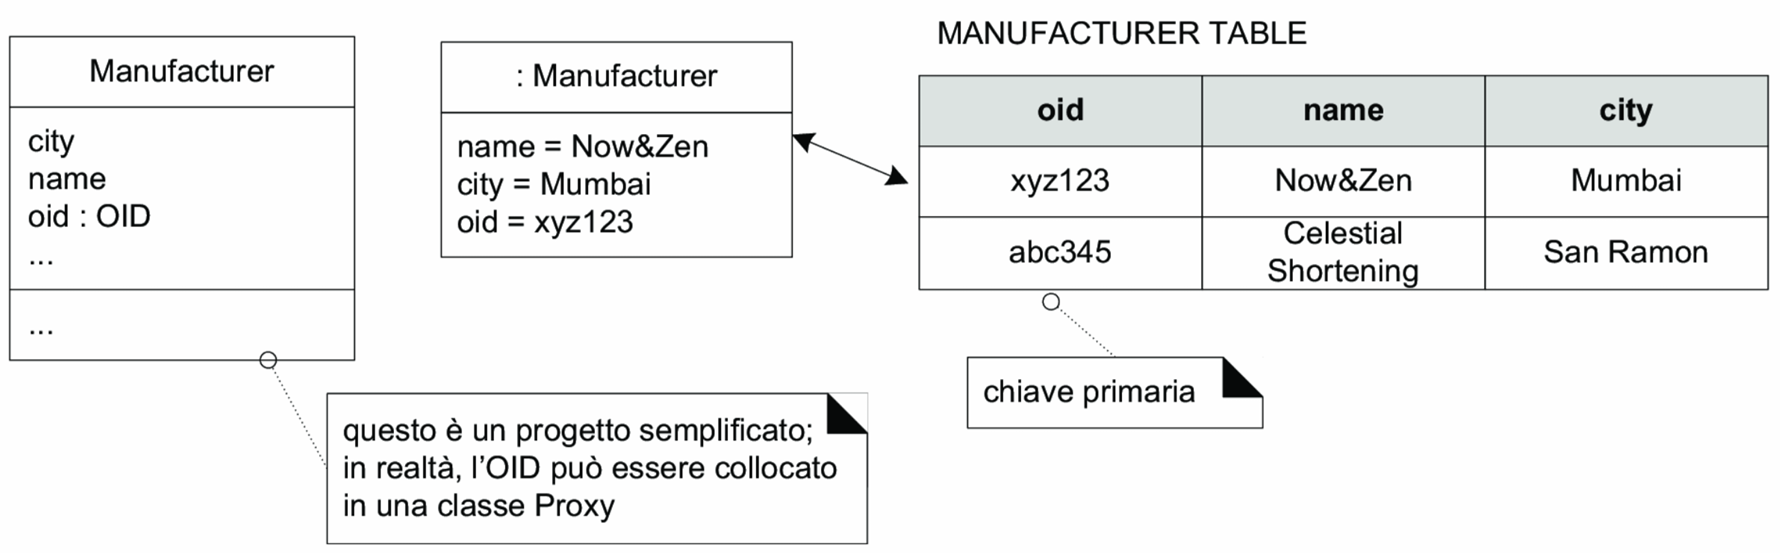
\includegraphics[scale=0.25]{Esercitazione - Design Patterns/Object Identifier.png}
    \end{center}
}

    \newpage
    \mysubsubsectionformatted{Accesso a un Servizio di Persistenza}
    Un pattern utile a fornire un unico punto di accesso è il \textbf{Facade}.
    \subsubsection{Design Pattern Facade}
    \myparagraph{
    \begin{tcolorbox}[colback=blue!5!white, colframe=blue!75!black]
        Il pattern fornisce un'interfaccia unificata ai servizi forniti di un certo sottosistema.
        La Facade delega le richieste provenienti dai client verso gli oggetti del sottosistema che nasconde. 
        Il suo intento è quello di rendere più semplice l'uso di un sottosistema.
    \end{tcolorbox}

    \vspace{0.1cm}
    \begin{center}
        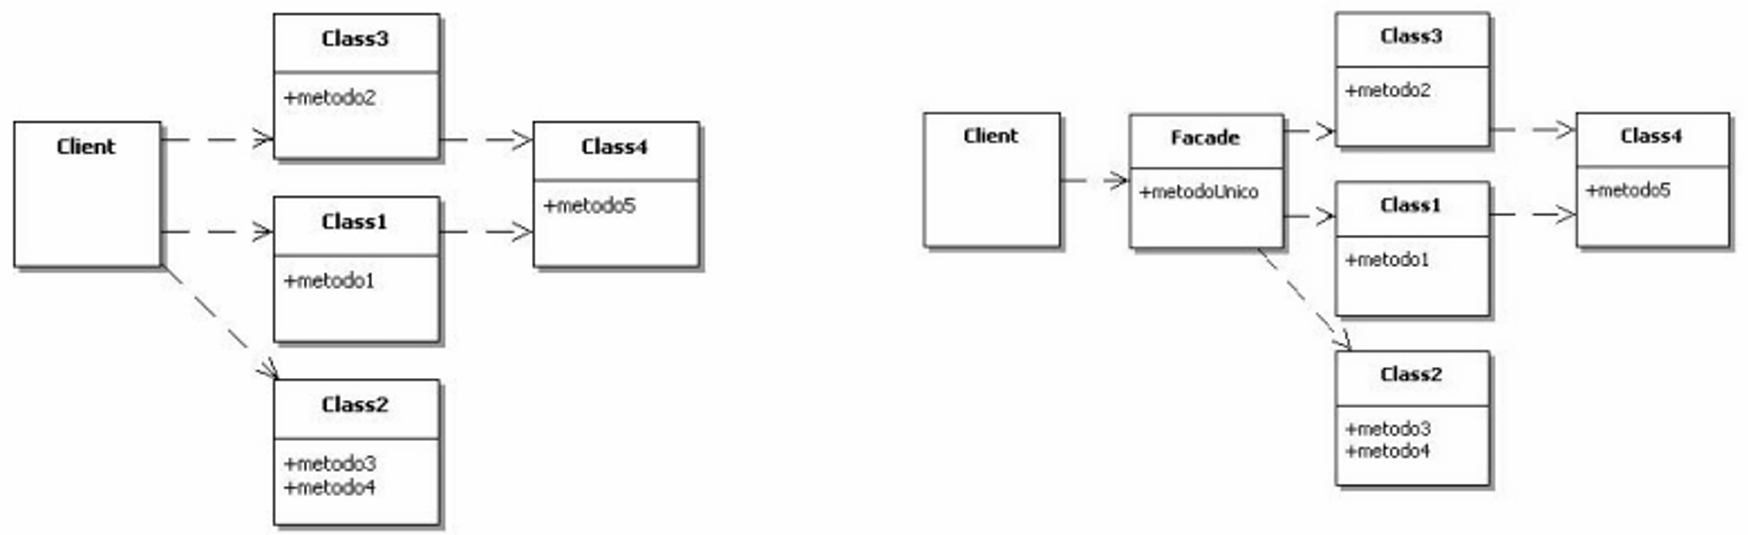
\includegraphics[scale=0.25]{Esercitazione - Design Patterns/Facade.png}
    \end{center}
    I partecipanti del pattern sono:
    \begin{enumerate}
        \item \textbf{Facade}: Conosce le classi responsabili per una richiesta e delega le richieste dei client
        agli oggetti appropriati del sottosistema.
        \item \textbf{Classi del sottosistema}: Implementano le funzionalità del sottosistema e gestiscono il lavoro
        assegnato dal Facade, questo però senza aver alcun riferimento di quest'ultima.
    \end{enumerate}

    Bisogna fare alcune considerazioni riguardo questo pattern:
    \begin{enumerate}
        \item Diminuisce l'accoppiamento tra client e sottosistema.
        \item Nasconde al client le componenti del sottosistema.
        \item Il client può comunque usare direttamente le classi del sottosistema.
    \end{enumerate}
    Si può anche rendere il Facade una classe astratta con sottoclassi concrete per diminuire ulteriormente
    l'accoppiamento. I client possono comunicare con il sottosistema mediante l'interfaccia della classe astratta Facade.

    \mysubsubsectionformatted{Facade vs Adapter}
    \begin{enumerate}
        \item Entrambi sono dei wrapper.
        \item Entrambi si basano su un'interfaccia, però:
        \item \begin{enumerate}
            \item Facade lo semplifica.
            \item Adapter lo converte.
        \end{enumerate}
    \end{enumerate}
}

    \mysubsubsectionformatted{Materializzazione e Dematerializzazione}
    In questa sezione vedremo \textbf{chi si occupa della Materializzazione e \\l'archiviazione degli oggetti}.

    Esistono due tipi di \textbf{Mapping}:
    \begin{enumerate}
        \item \textbf{Direct Mapping}: una classe che rappresenta un oggetto persistente \\definisce al suo interno il codice
              per il suo salvataggio nel DB (il codice è generato in automatico).
        \item \textbf{Indirect Mapping}: esistono classi apposite volte al recupero e al salvataggio dei dati in un DB.
    \end{enumerate}

    Questi due tipi di mappature si possono rappresentare mediante due pattern: \coloredtext[blue]{\textbf{Active Record}} per il Direct e \coloredtext[blue]{\textbf{Database Mapper}}
    per l'Indirect.

    \newpage
    \mysubsectionformatted{Active Record - Direct Mapping}
\myparagraph{
    \begin{tcolorbox}[colback=blue!5!white, colframe=blue!75!black]
        Il pattern architetturale permette di convertire ciascuna classe di dominio in tabella del DB.
        Combina i dati e il comportamento di un'entità in un'unica classe e inserisce la
        logica di accesso ai dati nell'oggetto di dominio, in modo che tutti sappiano come leggere e
        scrivere i dati da/al DB.
    \end{tcolorbox}
    
    \begin{center}
        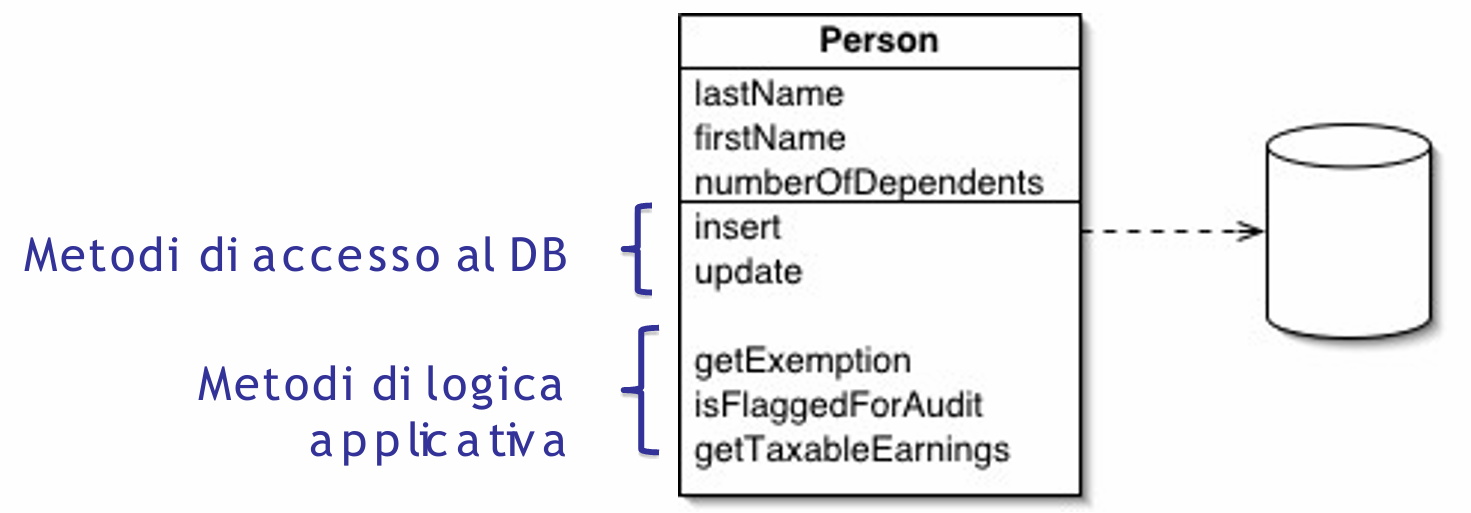
\includegraphics[scale=0.25]{Esercitazione - Design Patterns/Active Record.png}
    \end{center}

    Active Record fa uso di alcuni metodi e strutture dati:
    \begin{enumerate}
        \renewcommand{\labelenumii}{\arabic{enumi}.\arabic{enumii}}
        \item \textbf{Metodo load}: costruisce un'istanza partendo dai risultati generati da una query SQL.
        \item \textbf{Metodi finder} statici: incapsulano le query SQL e ritornano le istanze degli oggetti.
        \item \textbf{Costruttore classico}: costruisce nuove istanze da inserire successivamente nel DB.
        \item \textbf{Metodi di aggiornamento del DB}:
              \begin{enumerate}
                  \item \textbf{update}: aggiorna un record esistente con i valori degli attributi.
                  \item \textbf{insert}: aggiunge un record utilizzando i valori degli attributi.
                  \item \textbf{delete}: elimina il record corrispondente dell'oggetto corrente.
              \end{enumerate}
        \item \textbf{Metodi accessors}:
              \begin{enumerate}
                  \item I metodi \textbf{set} e \textbf{get} per accede ai campi.
                  \item Effettuano la conversione dei dati per memorizzare i valori degli attributi in un formato SQL-oriented.
                  \item Possono richiedere un'immediata sincronizzazione del DB.
              \end{enumerate}
        \item \textbf{Metodo di logica di business}
    \end{enumerate}
    \vspace{0.1cm}

    \resizebox{\columnwidth}{!}{%
        \begin{tabular}{l|l|}
            \hline
            \rowcolor[HTML]{32CB00}
            \multicolumn{1}{|c|}{\cellcolor[HTML]{32CB00}\textbf{Vantaggi}} & \multicolumn{1}{c|}{\cellcolor[HTML]{FE0000}\textbf{Svantaggi}}                                                                                     \\ \hline
            \multicolumn{1}{|l|}{Semplice da implementare e usare}          & \begin{tabular}[c]{@{}l@{}}L'accoppiamento fra la logica applicativa e il DB\\ rende difficile il refactoring dei due progetti\end{tabular}         \\ \hline
                                                                            & \begin{tabular}[c]{@{}l@{}}Si cerca di mantenere una corrispondenza stretta (o quasi)\\ fra lo schema del DB e l'entità del modello OO\end{tabular} \\ \cline{2-2}
        \end{tabular}%
    }
}
    \newpage
    \mysubsectionformatted{Database Mapper - Indirect Mapping}
\myparagraph{
    \begin{tcolorbox}[colback=blue!5!white, colframe=blue!75!black]
        Il framework (o pattern di progettazione) permette di definire una classe che si occupi della gestione dei processi
        di materializzazione da un DB, la dematerializzazione della memoria verso il DB e
        il caching degli oggetti con l'obiettivo di aumentare la performance del sistema.
    \end{tcolorbox}

    Il pattern definisce un DB Mapper per ogni classe di oggetti persistenti, possono esistere diversi
    tipi di Mapper a seconda dei meccanismi di memorizzazione.

    \begin{center}
        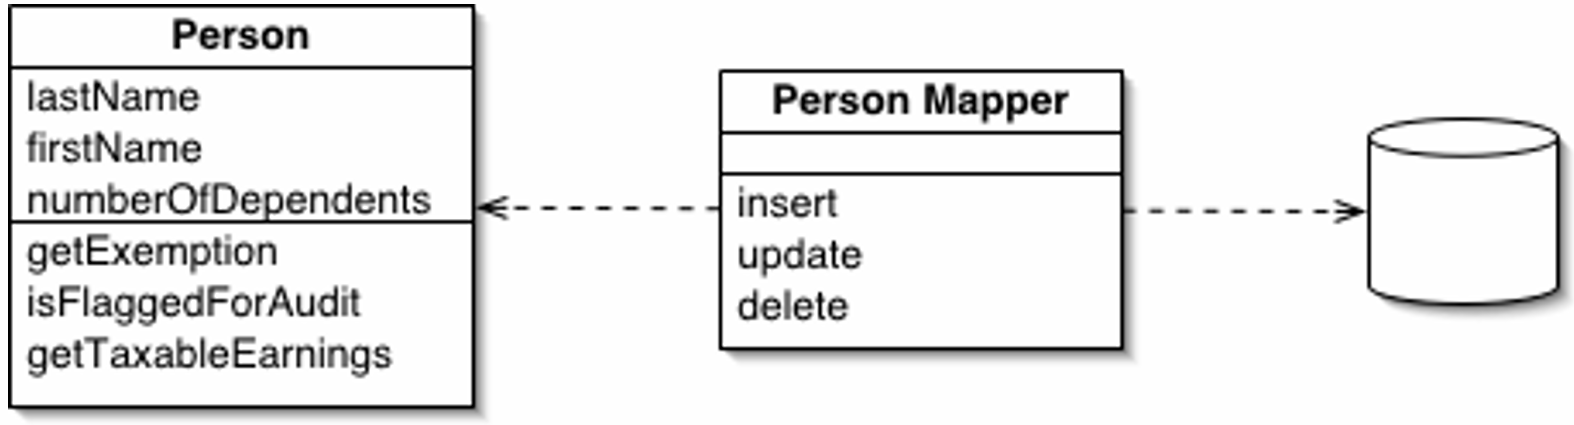
\includegraphics[scale=0.25]{Esercitazione - Design Patterns/Database Mapper.png}
    \end{center}

    \textbf{Person Mapper} è uno strato separato di componenti dedicati a trasferire i dati fra l'applicazione
    (\textbf{Person}) e il \textbf{Database}, trattando indipendentemente i due schemi (OO e ER). Infatti, la
    logica di business è inconsapevole dell'esistenza del Database.\\
    Generalmente, il pattern ne coinvolge di ulteriori per la gestione della sincronizzazione fra i due schemi
    (es. \textit{UnitOfWork} o \textit{IdentityMap}).\\
    Usiamo questo pattern per \textbf{gestire un mapping complesso fra DB e logica di business}.

    \begin{center}
        \resizebox{\columnwidth}{!}{%
            \begin{tabular}{ll}
                \hline
                \rowcolor[HTML]{32CB00}
                \multicolumn{1}{|c|}{\cellcolor[HTML]{32CB00}\textbf{Vantaggi}} & \multicolumn{1}{c|}{\cellcolor[HTML]{FE0000}\textbf{Svantaggi}} \\ \hline
                \multicolumn{1}{|l|}{Isola totalmente i due strati}             & \multicolumn{1}{l|}{Difficolta nell'implementazione}            \\ \hline
                                                                                &
            \end{tabular}%
        }
    \end{center}
    \newpage
}

    \mysubsectionformatted{Materializzazione in cache}
    Vogliamo mantenere all'interno della cache locale gli oggetti che sono stati materializzati in modo da:
    \begin{enumerate}
        \item Aumentare le prestazioni
        \item Supportare la gestione delle transazioni
    \end{enumerate}

    Il pattern utile allo scopo è il \coloredtext[blue]{\textbf{Cache Management}}
    \mysubsubsectionformatted{Design Pattern Cache Management}
    \myparagraph{
    \begin{tcolorbox}[colback=blue!5!white, colframe=blue!75!black]
        Il pattern estende il design pattern \textbf{Database Mapper}, facendo si che siano
        responsabili per la gestione della cache. Ogni Mapper può mantenere e gestire una propria
        cache privata. Il pattern verifica prima di tutto se gli oggetti sono in cache
        prima di recuperarli dal DB per evitare materializzazioni inutili.
    \end{tcolorbox}
}
    L'algoritmo di materializzazione, in pseudocodice, è strutturato in questo modo:
    \vspace{-0.1cm}
    \begin{algorithm}
        \caption{Gestione Cache}
        \begin{algorithmic}[1]
            \If{l'oggetto è in cache}
            \State ritorna l'oggetto
            \Else
            \State materializza l'oggetto dal database
            \State salva l'oggetto in cache
            \State ritorna l'oggetto
            \EndIf
        \end{algorithmic}
    \end{algorithm}
    \vspace{-0.1cm}

    Per progettare questa funzionalità, il pattern utile allo scopo è il \textbf{Template Method} (visto nella prima esercitazione).
    Il template method sarà il metodo \textbf{get} in una superclasse astratta. Ogni mapper specifico darà poi la sua implementazione
    di come ottenere i propri oggetti dal repository.

    \setcounter{figure}{0}
    \begin{figure}[H]
        \caption{Template Method per la materializzazione}
        \centering
        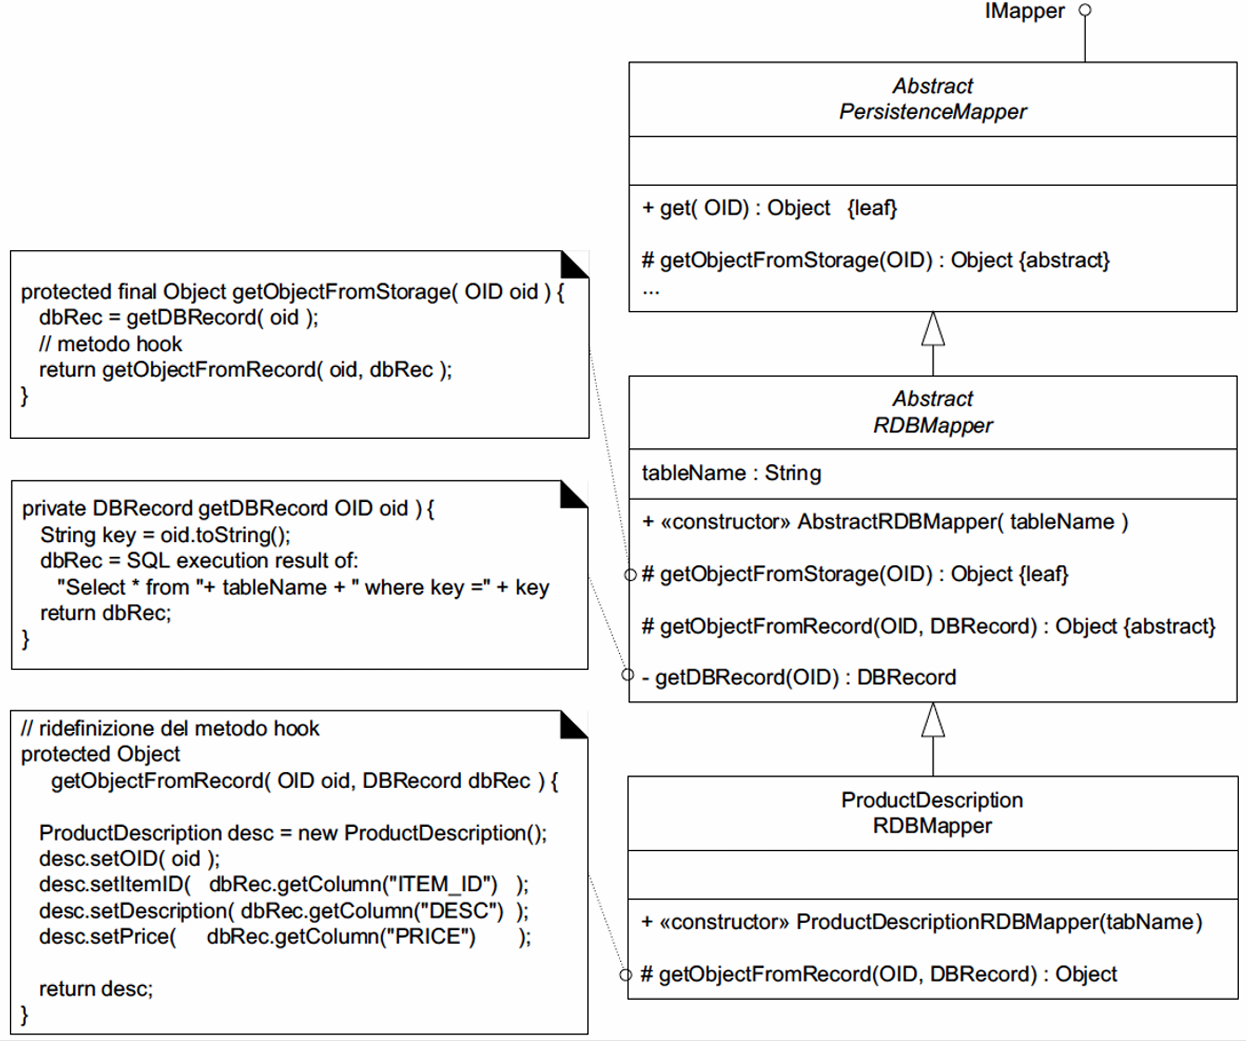
\includegraphics[scale=0.18]{Esercitazione - Design Patterns/Template Method Materializzazione.png}
    \end{figure}

    \newpage
    Fino ad'ora, le query SQL sono sempre state inserite dentro al codice dei metodi.

    \begin{center}
        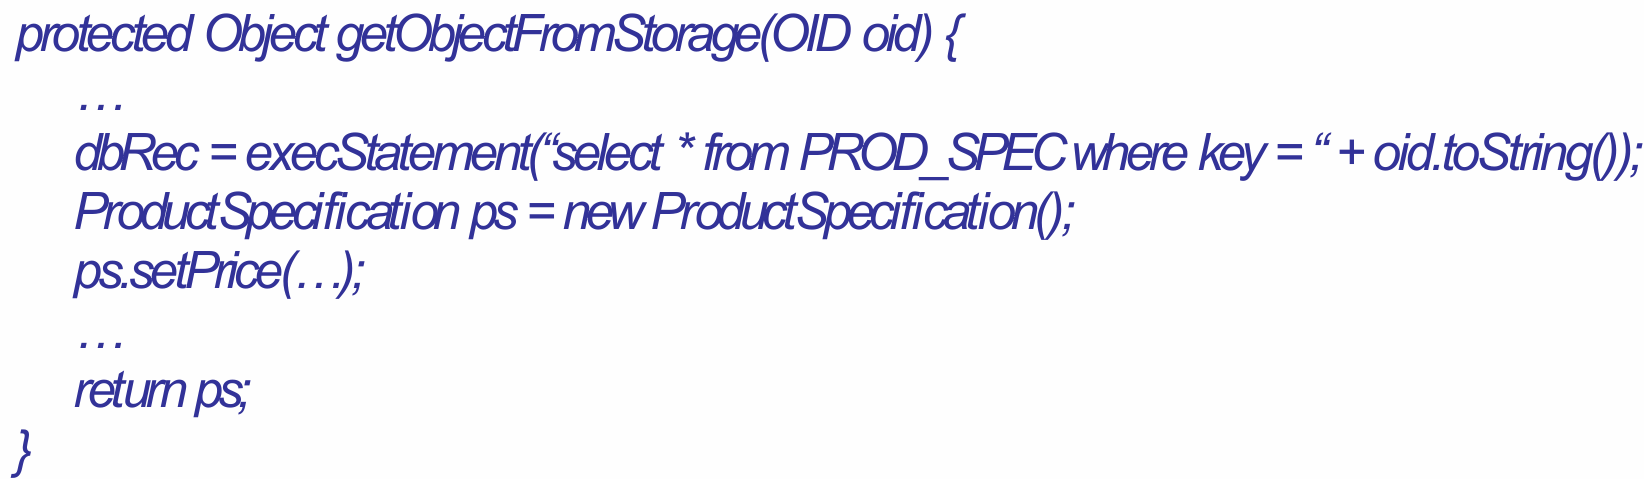
\includegraphics[scale=0.25]{Esercitazione - Design Patterns/Template Method SQL/Fase 1.png}
    \end{center}

    Per migliorare l'implementazione,
    si può mantenere una classe \textbf{Singleton} dove memorizzare tutte le query SQL necessarie (RDBOperations).

    \begin{center}
        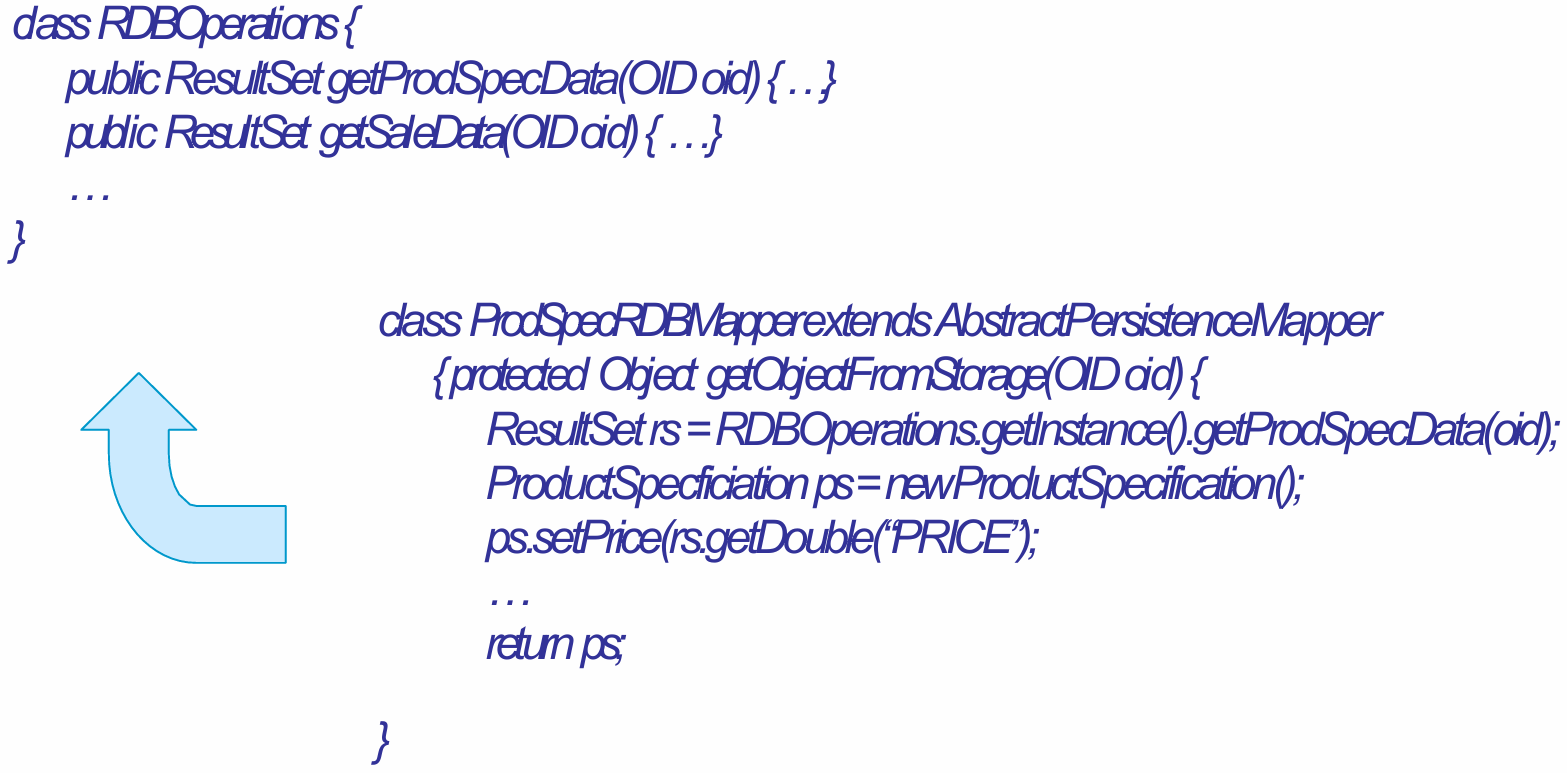
\includegraphics[scale=0.25]{Esercitazione - Design Patterns/Template Method SQL/Fase 2.png}
    \end{center}

    Risulta vantaggioso isolare le query in modo da rendere più facile la manutenzione migliorare la performance.
    \newpage
    }